\chapter{Evaluation on a corporate dataset}\label{chap:cisco-dataset}

The tree methods were finally evaluated on a corporate dataset in the domain of computer security. It is reasonable to expect the methods to perform similarly to their behaviour on the publicly available datasets. However, this task is significantly harder, which influences each method differently.

\section{The used dataset}

The models were evaluated on a proprietary dataset provided by Cisco Cognitive Intelligence, consisting of records of network connections from clients (e.g. user computers or mobile devices) to some on-line services. The dataset represents HTTP traffic of more than 100 companies. Two datasets were collected, each spanning 1 day of traffic. The training data was traffic from 2019-11-18, while the data used for testing was collected the following day, 2019-11-19. For each connection, a proprietary classification system based on \cite{jusko_graph-based_2017} provided labels, classifying the connections either as legitimate or malicious (connected to malware activity). The data was sampled to include 90\% of negative bags and 10\% of positive bags. Table \ref{tab:cisco-features} lists all the features provided in the dataset for each connection.

\begin{table}{h}
  \centering
  \begin{tabular}{l}
    \toprule
    The duration of the connection \\
    The client port number \\
    The IANA assigned internet protocol number \\
    The server port number \\
    The number of bytes sent from the client to the server \\
    The number of bytes sent from the server to the client \\
    The number of packets sent from the client to the server \\
    The number of packets sent from the server to the client \\
    The number of individual TCP connections \\
    The number of SYN packets sent from the client to the server \\
    The number of SYN-ACK packets sent from the server to the client \\
    The number of RST packets sent from the client to the server \\
    The number of RST packets sent from the server to the client \\
    The number of FIN packets sent from the client to the server \\
    The number of FIN packets sent from the server to the client \\
    \bottomrule
  \end{tabular}
  \caption{The information provided for each connection in the corporate dataset.}\label{tab:cisco-features}
\end{table}

In addition to that, each connection contains the URL the client is connecting to. A hierarchical representation of the URL using MIL was added to the features -- the MIL framework is powerful enough to enable a mix of traditional and MIL-based features. The URL model is based on the previous works \cite{dedic_hierarchicke_2017} and \cite{pevny_nested_2020}. The hierarchical model is visualized in figure \ref{fig:URL-model}.


\begin{figure}[H]
  \centering
  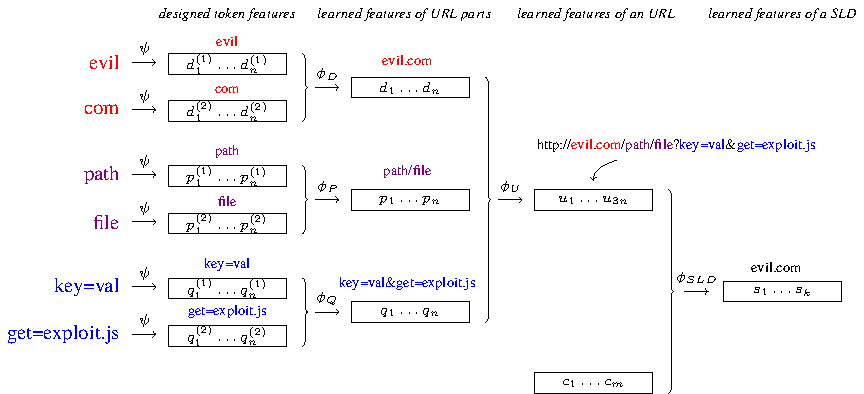
\includegraphics[width=\textwidth]{images/URL-model/URL-model.pdf}
  \caption{Hierarchical model of a URL. The vector \( c_1, \dots, c_m \) represents the connection features.}\label{fig:URL-model}
\end{figure}

\section{Used models}

The models for evaluation were implemented in the Julia programming language (see \cite{bezanson_julia:_2017}) using the Flux.jl framework for machine learning (see \cite{innes_flux:_2018}) and the Mill.jl framework for multi-instance learning (see \cite{pevny_milljl_2019}).

The embedding \( \phi \) was realised by a MIL neural network. Using the notation from figure \ref{fig:URL-model}, \( \phi_D \), \( \phi_P \) and \( \phi_Q \) consisted of a layer of 20 neurons, followed by concatenating element-wise mean and element-wise maximum of all instances in a bag. After joining the URL parts by concatenating their representations, \( \phi_U \) consisted of a layer of 120 neurons, followed by concatenation with the 15 connection features. Finally, \( \phi_\mathrm{SLD} \) consist of a layer of 135 neurons, followed by aggregation by concatenating element-wise mean and element-wise maximum of all instances in a bag, followed by a layer with 270 neurons. All the neurons used the ReLU activation function (see \cite{hahnloser_digital_2000}). Layer weights were initialized using Glorot initialization (see \cite{glorot_understanding_2010}), bias vectors were initialized to zeros. ADAM (see \cite{kingma_adam:_2014}) was used as the optimization method. The models were trained using 20 mini-batches of 50 bags each.

A mean model and a classification model have been constructed similarily to the ones in section \ref{sec:baseline-models}
The classification model is identical, with a final output layer of 2 neurons added. ADAM was used as the optimization method optimizing the cross-entropy loss. The accuracy of the model has been evaluated by selecting the optimal threshold on its output.

\section{Multi-class classification}
Apart from the task of learning a clustering based on a two-class labeling of bags as either legitimate or malicious, a multi-class classification system was also trained and evaluated. In this case, the data points were labeled as either legitimate or belonging to one of 19 classes of malware, described in table \ref{tab:cisco-malware-classes}.

\begin{table}{h}
  \centering
  \begin{tabular}{l}
    \toprule
    Legitimate traffic \\
    Ad injector \\
    Anonymization software \\
    Advanced Persistent Threat (APT) \\
    Banking trojan \\
    Click fraud \\
    Cryptocurrency miner \\
    Data exfiltration \\
    Exploit kit \\
    Information stealer \\
    Malicious advertising \\
    Malicious content distribution \\
    Malware distribution \\
    Money scam \\
    Potentially unwanted application (PUA) \\
    Ransomware \\
    Scareware \\
    Spam botnet \\
    Spam tracking \\
    Trojan \\
    \bottomrule
  \end{tabular}
  \caption{The malware classes distinguished in the multi-class dataset.}\label{tab:cisco-malware-classes}
\end{table}

The data was sampled to include 81\% of legitimate bags and 1\% of every other class.

\section{Method comparison}

Figure \ref{fig:cisco-ratio} shows the value of \( \mathrm{silhouette} \left( \cdot \right) \) for all the methods over the learning period. Table \ref{tab:cisco-accuracy} shows the accuracy of the final model for each method. Figure \ref{fig:cisco-kNN-poly} shows the relation between the number of data points used to seed the kNN classifier and its accuracy. Due to the high noise (even when averaging over three runs), in this figure the values are fitted by a polynomial of order 4 so that they could be compared. The original values are plotted in the appendix.

Figure \ref{fig:cisco-multiclass-ratio} shows the value of \( \mathrm{silhouette} \left( \cdot \right) \) for all the methods for the 20-class classification problem over the learning period. Table \ref{tab:cisco-accuracy} shows the accuracy of the final model for each method. Figure \ref{fig:cisco-multiclass-kNN-poly} shows the relation between the number of data points used to seed the kNN classifier and its accuracy. Due to the high noise (even when averaging over three runs), in this figure the values are fitted by a polynomial of order 4 so that they could be compared. The original values are plotted in the appendix.

\begin{figure}[H]
  \centering
  \begin{subfigure}[t]{0.49\textwidth}
    \centering
    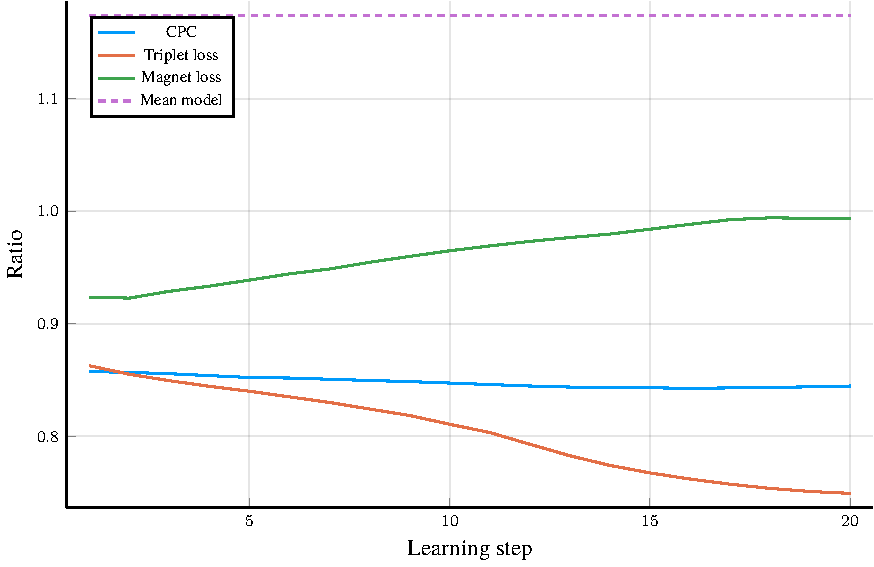
\includegraphics[width=\textwidth]{images/cisco/ratio/cisco-ratio.pdf}
    \caption{The value of \( \mathrm{silhouette} \left( \cdot \right) \) over the learning period.}\label{fig:cisco-ratio}
  \end{subfigure}
  \hfill
  \begin{subfigure}[t]{0.49\textwidth}
    \centering
    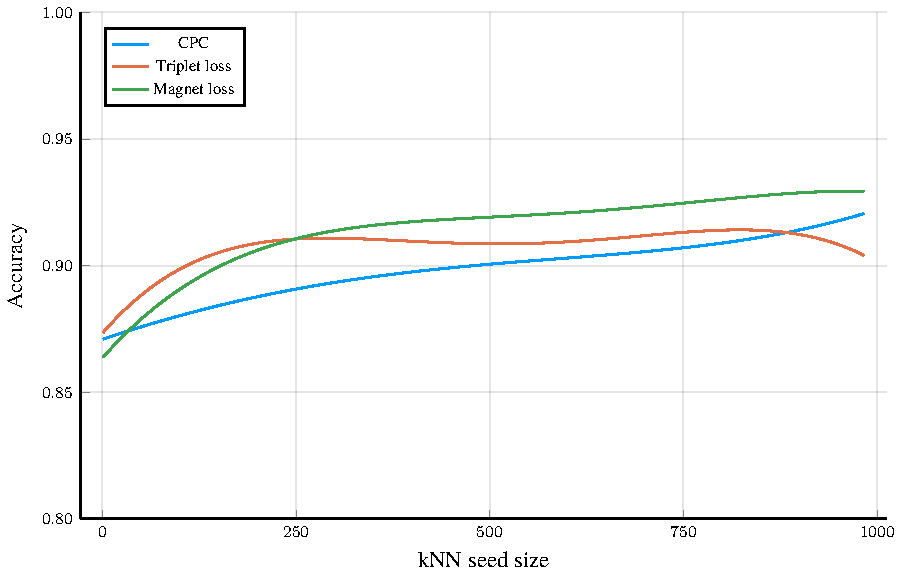
\includegraphics[width=\textwidth]{images/cisco/kNN-poly/cisco-kNN-poly.pdf}
    \caption{The accuracy of a kNN classifier built on the final embedding as a function of the number of samples used to seed it. Average of three runs, fitted by a polynomial curve.}\label{fig:cisco-kNN-poly}
  \end{subfigure}
  \caption{The performance metrics for two class classification on the corporate dataset.}
\end{figure}

\begin{figure}[H]
  \centering
  \begin{subfigure}[t]{0.49\textwidth}
    \centering
    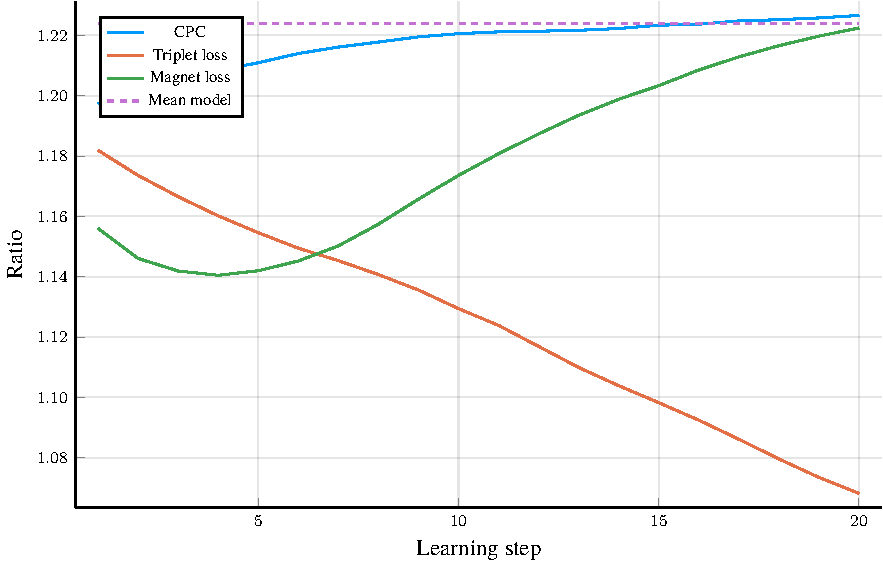
\includegraphics[width=\textwidth]{images/cisco-multiclass/ratio/cisco-multiclass-ratio.pdf}
    \caption{The value of \( \mathrm{silhouette} \left( \cdot \right) \) over the learning period.}\label{fig:cisco-multiclass-ratio}
  \end{subfigure}
  \hfill
  \begin{subfigure}[t]{0.49\textwidth}
    \centering
    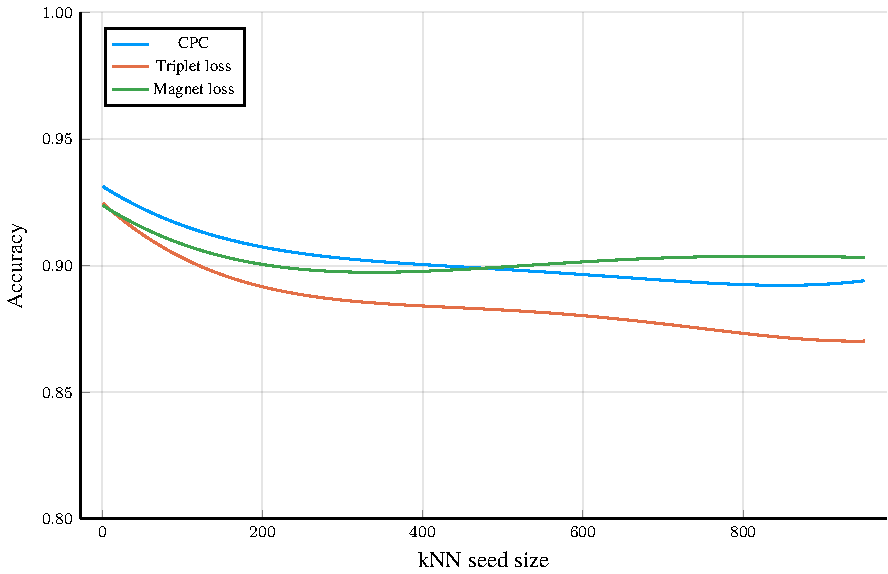
\includegraphics[width=\textwidth]{images/cisco-multiclass/kNN-poly/cisco-multiclass-kNN-poly.pdf}
    \caption{The accuracy of a kNN classifier built on the final embedding as a function of the number of samples used to seed it. Average of three runs, fitted by a polynomial curve.}\label{fig:cisco-multiclass-kNN-poly}
  \end{subfigure}
  \caption{The performance metrics for twenty class classification on the corporate dataset.}
\end{figure}

\begin{table}
  \centering
  \begin{tabular}{lrrr}
    \toprule
    Classification problem & CPC   & Triplet loss & Magnet loss \\
    \midrule
    2 classes              & 0.920 & 0.910        & \textbf{0.930} \\
    20 classes             & 0.893 & 0.868        & \textbf{0.904} \\
    \bottomrule
  \end{tabular}
  \caption{The accuracy of the final models for the corporate datasets.}\label{tab:cisco-accuracy}
\end{table}

As can be seen from the figures and the table, for this problem, magnet loss performed the best. The model based on contrastive predictive coding is the second best and for the model based on triplet, the value of \( \mathrm{silhouette} \left( \cdot \right) \) actually goes down over the learning period. Figure \ref{fig:cisco-kNN-poly} shows that triplet loss and magnet loss reach their peak performance for a small number of seed data, but CPC improves its performance with every new seed point. For the multi-class version of the experiment, magnet loss still leads in terms of accuracy, but is somewhat surprisingly surpassed by CPC in terms of \( \mathrm{silhouette} \left( \cdot \right) \). Figure \ref{fig:cisco-multiclass-kNN-poly} shows an inverse relationship than expected, but this can be explained by the high number of classes which are only sampled for a sufficient number of seed data points.
